\section{663 --- Equal Tree Partition}
Given a binary tree with n nodes, your task is to check if it's possible to partition the tree to two trees which have the equal sum of values after removing exactly one edge on the original tree.

\paragraph{Example 1:}

\begin{flushleft}
\textbf{Input}:     

\begin{figure}[H]
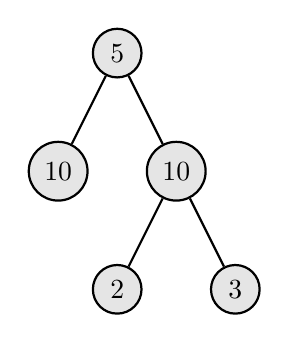
\begin{tikzpicture}
[every node/.style={draw, circle,
 minimum size=6mm, fill=gray!20!},
  node distance=8mm, 
  every join/.style={>=stealth,->},
 thick
]
\node{5}
child{node{10}}
child{node{10} child{node{2}} child{node{3}} };
\end{tikzpicture}
\end{figure}

\textbf{Output}:  \lstinline[language=C++, basicstyle=\small\ttfamily, keywordstyle=\bfseries\color{green!40!black}]|true|

\textbf{Explanation}: 

\begin{figure}[H]
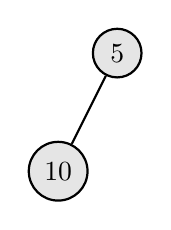
\begin{tikzpicture}
[every node/.style={draw, circle,
 minimum size=6mm, fill=gray!20!},
  node distance=8mm, 
  every join/.style={>=stealth,->},
 thick
]
\node{5}
child{node{10}}
child[missing];
\end{tikzpicture}
\end{figure}
    
Sum: 15

\begin{figure}[H]
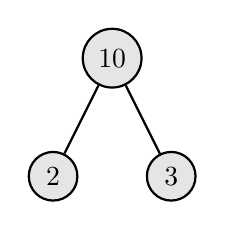
\begin{tikzpicture}
[every node/.style={draw, circle,
 minimum size=6mm, fill=gray!20!},
  node distance=8mm, 
  every join/.style={>=stealth,->},
 thick
]
\node{10}
child{node{2}}
child{node{3}};
\end{tikzpicture}
\end{figure}

Sum: 15
\end{flushleft}

\paragraph{Example 2:}
\begin{flushleft}


\textbf{Input}:     
\begin{figure}[H]
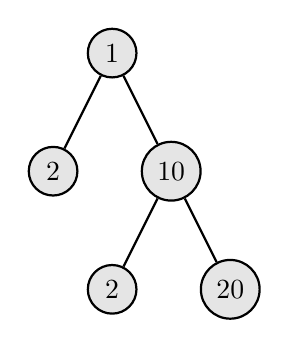
\begin{tikzpicture}
[every node/.style={draw, circle,
 minimum size=6mm, fill=gray!20!},
  node distance=8mm, 
  every join/.style={>=stealth,->},
 thick
]
\node{1}
child{node{2}}
child{node{10} child{node{2}} child{node{20}} };
\end{tikzpicture}
\end{figure}

\textbf{Output}:  \lstinline[language=C++, basicstyle=\small\ttfamily, keywordstyle=\bfseries\color{green!40!black}]|false|

\textbf{Explanation}: 

You can't split the tree into two trees with equal sum after removing exactly one edge on the tree.
\end{flushleft}

\paragraph{Note:}

\begin{itemize}
\item The range of tree node value is in the range of  \lstinline[language=C++, basicstyle=\small\ttfamily, keywordstyle=\bfseries\color{green!40!black}]|[-100000, 100000]|.
\item $1 \leq n \leq 10000$
\end{itemize}

\subsection{Depth First Search}
After removing a edge from parent to child, the subtree rooted at child must be half the sum of the entire tree.

We can put the sum of every subtree into an array by depth-first search. Then, we check if we can find a value inside the array which is half the sum of the entire tree.

In the implementation, we should pay attention to a few notes
\begin{itemize}
\item The sum of a subtree rooted at current node will be the current last element of the array.
\item The total sum of entire tree should be even number.
\item We need to remove last element of the array which is the total sum of entire tree. 
\end{itemize}
